\documentclass[../../main.tex]{subfiles}
\begin{document}

\subsection*{8.3}
Due fili indefiniti distanti 2a =4cm, paralleli all'asse x.
\\Calcolare il campo magnetic $\vec{B}(z)$ sull'asse dei due fili e a quale distanza dal centro O un piccolo ago magnetico orientato parallelo mentre $\vec{B}$ risente di una forza non nulla.
\\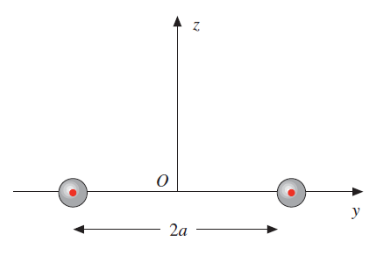
\includegraphics[scale=0.3]{e_8_3_0.png}
\\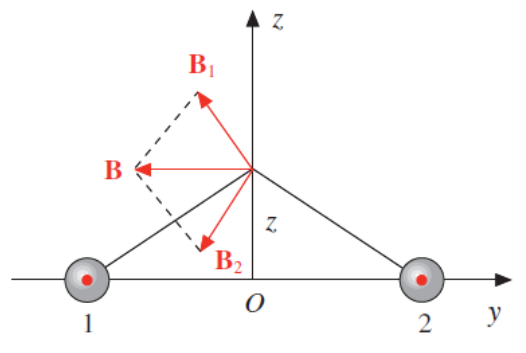
\includegraphics[scale=0.3]{e_8_3_1.png}
\subsubsection*{Formule utilizzate}
\subsubsection*{Soluzione punto a}
$B_{1z}+B_{2z} = B_z = 0$
\\$B_{1y} + B_{2y} = 2B_{1y} = B_y = 2(B_1\sin\alpha)$
\\$\vec{B}=2\frac{\mu_0 i}{2\pi\sqrt{a^2+z^2}}\sin\alpha\vec{u_y} = \frac{\mu_o i z}{\pi(a^2+z^2)}\vec{u_y}$
\\$\vec{F}=\nabla(\vec{m} * \vec{B})=\nabla(mBy)$
\\$F=m\frac{dBy}{dz}=0$
\\$\frac{dB}{dz}=\frac{\mu_0 i}{\pi}\frac{a^2+z^2-2z^2}{(a^2+z^2)^2} = 0$
\subsubsection*{Soluzione punto b}
\newpage

\end{document}